\chapter{Biogeochemical Heating and the Terrestrial Carbon Cycle}
\label{chapter:global_bomb}
\graphicspath{{global_bomb/figs/}}

\lettrine[lines=3,loversize=0.1,findent=-0.9em,nindent=0.5em,slope=0.6em]{A}{} vertical dimension was introduced into a model of the compost
bomb in \cref{chapter:continuous_compost_bomb}. It was shown that this doesn't
suppress the compost bomb. That analysis was local ---  the modelling was done at a single point on the Earth's surface. It would be interesting to see
what a globally-averaged model that included biogeochemical heating would predict. Work by~\cite{Cox2006} suggested that the terrestrial carbon cycle is stable
only for certain parameter ranges. 
In this chapter, I will explore the impact that biochemical heating has on the stability of the global climate-carbon cycle system
\section{Compost Bomb Bifurcation Analysis}

\subsection{Dynamical Equations}
The compost bomb equations, introduced by~\cite{Luke2011}, are
\begin{subequations}
  \label{eq:compost_bomb_equations}
  \begin{align}
    c \dv{T_s}{t} &= - \kappa \left(T_s - T_a\right) + Ar_0C_se^{\alpha T_s} \label{eq:compost_bomb_soil_temperature} \\
    \dv{C_s}{t} &= \Pi - r_0C_se^{\alpha T_s}, \label{eq:compost_bomb_soil_carbon}
  \end{align}
\end{subequations}
where $T_s$ and $C_s$ are soil temperature and carbon, $T_a$ is the atmospheric temperature, $\alpha = 0.1\log Q_{10}$ is the sensitivity of
temperature to respiration, $\Pi$ is Net Primary Productivity, $A$ is the heat released by respiration, $\kappa$ is a heat transfer coefficient,
$c$ is a heat capacity and $r_0$ is the specific rate of respiration.

While the analysis in~\cite{Luke2011} was local, it will be assumed that \cref{eq:compost_bomb_equations} hold at the global scale too, where quantities are
replaced by their global value. It will also be assumed that Net Primary Productivity, $\Pi$, is an increasing function of atmospheric \ce{CO2}, as is $T_a$. 

There is a timescale separation in \cref{eq:compost_bomb_equations}. The dynamic of soil carbon are relatively slow, with a soil turn over time measured in the decades \parencite{Varney2022},
whereas the dynamics of soil temperature are much faster, reaching an equilibrium with the air temperature on the time scale of a day \parencite{Best2005}. With this in mind, the soil
temperature can be set to equilibrium, as calculated by putting \cref{eq:compost_bomb_soil_temperature} equal to zero. This gives
\begin{equation*}
  0 = - \kappa \left(T_s - T_a\right) + Ar_0C_se^{\alpha T_s}
\end{equation*}
which can be solved for the soil temperature
\begin{equation}
  \label{eq:soil_temperature_equilibrium}
  T_s = T_a - \frac{1}{\alpha} W\left(-\frac{Ar_0C_s \alpha e^{\alpha T_a}}{\kappa} \right),
\end{equation}
where $W(x)$ is the Lambert $W$ function \parencite{Corless1996}. The Lambert $W$ function, plotted in \cref{fig:lambert_W}, is defined as the solution to the equation
\begin{equation}
  \label{eq:lambert_W}
  W(x)e^{W(x)} = x.
\end{equation}
This function is multivalued, and the larger (less negative) of the two possible values should be taken, which corresponds to the smaller value of $T_s$, which is the stable solution.
\begin{figure}
  \centering
  \begin{tikzpicture}
    \begin{axis}[
      %xmin=-1,
      %xmax=4,
      enlarge y limits=true,
      enlarge x limits=true,
      axis lines=middle,
      xlabel=$x$,
      xlabel style={xshift=0.5cm, yshift=-0.2cm},
      ylabel=$W(x)$,
      ylabel style={xshift=-0.5cm, yshift=1.0cm},
      samples=500]
      \addplot[domain=-4.2:-1,color=black] (x * exp(x), x);
      \addplot[domain=-1:1,color=black] (x * exp(x), x);
    \end{axis}
  \end{tikzpicture}
  \caption[The Lambert $W$ function]{The Lambert $W$ function, for $x \in [-1/e,e]$. The minimum value of $x$ for which $W(x)$ is real is $-1/e$. For $x < 0$, $W(x)$ is
  multivalued.}
  \label{fig:lambert_W}
\end{figure}

After noting that the argument of $W$ is dimensionless, and that $r_0C_s$ has units of Net Primary Productivity, the quantity 
\begin{equation}
  \label{eq:critical_npp}
  \Pi_c = \frac{\kappa}{\alpha A}
\end{equation}
can be defined, which measures the influence of biogeochemical heating. No biogeochemical heating occurs for $A = 0$ or, equivalently, for $\Pi_c = \infty$. Similarly
biogeochemical heating is strongest for $A \rightarrow \infty$ or, again equivalently, for $\Pi_c = 0$.

\Cref{eq:soil_temperature_equilibrium} can now be rewritten as
\begin{equation}
  \label{eq:soil_temperature_equilibrium_nppc}
  T_s = T_a - \frac{1}{\alpha} W\left(-\frac{r_0C_s e^{\alpha T_a}}{\Pi_c} \right).
\end{equation}
\Cref{eq:soil_temperature_equilibrium_nppc} was then inserted into \cref{eq:compost_bomb_soil_carbon} to give
\begin{equation}
  \label{eq:soil_carbon_evolution}
  \dv{C_s}{t} = \Pi + \Pi_c W\left(-\frac{r_0C_s e^{\alpha T_a}}{\Pi_c} \right).
\end{equation}
which for given $\Pi$ and $T_a$ determines the evolution of $C_s$.

The implied equilibrium value for $C_s$ occurs when \cref{eq:soil_carbon_evolution} is zero. The value of $C_s$ for which this is true is
\begin{equation}
  \label{eq:equilibrium_soil_carbon_pic}
  C_s^{\mathrm{eq}} = \frac{\Pi}{r_0} e^{-\alpha T_a} e^{-\Pi/\Pi_c}.
\end{equation}
The no biogeochemical heating case can be recovered by sending $\Pi_c \rightarrow \infty$ which gives $C_s^{\mathrm{eq}} = \Pi/r_0$.

\subsection{Closing the System}
It has been stated that $T_a$ and $\Pi$ are functions of atmospheric carbon, so determining their behaviours requires specifying the behaviour of the rest of the carbon
cycle. The total carbon in the carbon cycle is conserved and so
\begin{equation}
  \label{eq:carbon_conservation}
  C_s + C_a + C_o = C_s^{\mathrm{eq}} + C_{a0} + C_{o0}
\end{equation}
where $C_a$ and $C_o$ are atmospheric and oceanic carbon and the quantities on the right-hand side are the equilibrium values.
Following~\cite{Cox2006}, it will be assumed that a fixed fraction, $\chi_0$, of atmospheric emissions reach the ocean, meaning
\begin{equation}
  \label{eq:simple_ocean}
  C_a = C_{a0} -\frac{1}{1+\chi_0} (C_s - C_{s}^{\mathrm{eq}}).
  %C_s = C_{s}^{\mathrm{eq}} - (1 + \chi_0)(C_a - C_{a0}.
\end{equation}
In the rest of this chapter it will be assumed that $\chi_0 = 1/4$, on the grounds that roughly half of atmospheric emissions remain in the atmosphere \parencite{Jones2005}
with the other half split approximately evenly between the land and the ocean \parencite{Friedlingstein2022}.

Making the further assumption that atmospheric temperatures scale logarithmically with atmospheric \ce{CO2} \parencite{Pierrehumbert2010} gives
\begin{equation}
  \label{eq:atmospheric_temperatures}
  T_a = \frac{S}{\log 2} \log \frac{C_a}{C_{a0}} 
\end{equation}
where $S$ is the effective climate sensitivity experienced by the soils. Substituting \cref{eq:atmospheric_temperatures} into \cref{eq:soil_carbon_evolution} 
leads to
\begin{equation}
  \label{eq:global_soil_carbon}
  \dv{C_s}{t} = \Pi(C_a) + \Pi_c W\left(-\frac{r_0C_s}{\Pi_c} \left(\frac{C_a}{C_{a0}}\right)^\mu \right),
\end{equation}
where
\begin{equation}
  \label{eq:mu_definition}
  \mu = \frac{\alpha S}{\log 2}
\end{equation}
and $C_a$ is determined through \cref{eq:simple_ocean}. By definition, $C_s = C_s^{\mathrm{eq}}$ when the left hand side of \cref{eq:global_soil_carbon} is set equal to zero.
This will correspond to a pre-industrial equilibrium when $C_a = C_{a0}$. This requires that 

\begin{equation}
  r_0 = \frac{\Pi_0}{C_s^{\mathrm{eq}}}e^{-\Pi_0/\Pi_c}, 
\end{equation}
where $\Pi_0 = \Pi\left(C_{a0}\right)$ is the NPP during the pre-industrial period.


\subsection{Computation of Bifurcation Point}
\label{sec:computation_of_bifurcation_point}
The stability of the equilibrium at $C_s = C_s^{\mathrm{eq}}$ is determined by the Jacobian of \cref{eq:global_soil_carbon}, which in this case amounts to
taking the derivative of the right-hand side of \cref{eq:global_soil_carbon} when $C_s = C_s^{\mathrm{eq}}$. The system will transition from being stable to unstable when
\begin{equation*}
  \dv{\dot{C_s}}{C_s} = 0.
\end{equation*}
In order to calculate the derivative the identity
\begin{equation}
  \label{eq:derivative_of_lambert_W}
  W'(x) = \frac{W(x)}{x\left(1 + W\left(x\right)\right)}
\end{equation}
will be useful, which follows from taking the derivative of \cref{eq:lambert_W}.

If the derivative of the right hand side of \cref{eq:global_soil_carbon} is taken and set to zero, 
\begin{equation}
  \label{eq:soil_carbon_lambda}
  \dv{\Pi}{C_a}\dv{C_a}{C_s} + \frac{\Pi_c}{C_s^{\mathrm{eq}}} \frac{W\left(-\frac{r_0C_s^{\mathrm{eq}}}{\Pi_c}\right)}{1+W\left(-\frac{r_0C_s^{\mathrm{eq}}}{\Pi_c}\right)} \left(
    1 + \mu \frac{C_s^{\mathrm{eq}}}{C_{a0}} \dv{C_a}{C_s}\right) = 0
\end{equation}
is obtained. This can be rearranged for $\mu$ to give
\begin{equation}
  \label{eq:critical_mu}
  \mu = -\frac{C_{a0}}{C_{s}^{\mathrm{eq}}}\dv{C_s}{C_a}\left(\dv{\Pi}{C_a}\dv{C_a}{C_s} \frac{C_s^{\mathrm{eq}}}{\Pi_c}\frac{1+W\left(-\frac{r_0C_s^{\mathrm{eq}}}{\Pi_c}\right)}{W\left(-\frac{r_0C_s^{\mathrm{eq}}}{\Pi_c}\right)} + 1 \right)
\end{equation}
which simplifies to
\begin{equation}
  \label{eq:critical_mu_simple_ocean}
  \mu = \left(1+\chi_0\right) \frac{C_{a0}}{C_{s}^{\mathrm{eq}}} -
  \frac{C_{a0}}{\Pi_c}\frac{1+W\left(-\frac{r_0C_s^{\mathrm{eq}}}{\Pi_c}\right)}{W\left(-\frac{r_0C_s^{\mathrm{eq}}}{\Pi_c}\right)}\dv{\Pi}{C_a}.
\end{equation}
This can be further reduced, by using \cref{eq:equilibrium_soil_carbon_pic}, to
\begin{equation*}
  \mu = \left(1+\chi_0\right) \frac{C_{a0}}{C_{s}^{\mathrm{eq}}} -
  \frac{C_{a0}}{\Pi_c}
  \frac{1+W\left(-\frac{\Pi_0}{\Pi_c}\exp\left(-\frac{\Pi_0}{\Pi_c}\right)\right)}
  {W\left(-\frac{\Pi_0}{\Pi_c}\exp\left(-\frac{\Pi_0}{\Pi_c}\right)\right)}\dv{\Pi}{C_a} 
\end{equation*}
and then by using the definition of the Lambert $W$ function, \cref{eq:lambert_W}, to give
\begin{equation*}
  \mu = \left(1+\chi_0\right) \frac{C_{a0}}{C_{s}^{\mathrm{eq}}} -
  \frac{C_{a0}}{\Pi_c}
  \frac{1-\frac{\Pi_0}{\Pi_c}}{-\frac{\Pi_0}{\Pi_c}}\dv{\Pi}{C_a}.
\end{equation*}
This can then be cleaned up to give a final form for the critical $\mu$ value, notated as $\mu^*$, which separates stable from unstable soil
carbon states. $\mu^*$ is therefore
\begin{equation}
  \label{eq:critical_mu_simple_ocean_in_terms_of_npp}
  \mu^* = \left(1+\chi_0\right) \frac{C_{a0}}{C_{s}^{\mathrm{eq}}} +
  \frac{C_{a0}}{\Pi_0} \dv{\Pi}{C_a} - \frac{C_{a0}}{\Pi_c}\dv{\Pi}{C_a}.
\end{equation}
It is instructive to take the $\Pi_c \rightarrow \infty$ limit, which gives the behaviour in the no biogeochemical heating case:
\begin{equation}
  \label{eq:mu_infinity}
  \mu^*_{\infty} =\left(1+\chi_0\right) \frac{C_{a0}}{C_{s}^{\mathrm{eq}}} +
  \frac{C_{a0}}{\Pi_0} \dv{\Pi}{C_a}.
\end{equation}
Therefore the effect of biogeochemical heating is the reduce the critical $\mu$ value for which an instability occurs by the amount
\begin{equation}
  \label{eq:reduction_in_stability_due_to_biogeochemical}
  \frac{C_{a0}}{\Pi_c}\dv{\Pi}{C_a}.
\end{equation}
When $\Pi_c \rightarrow 0$ this reduction becomes infinite and no stable soil carbon state is possible.

\Cref{eq:critical_mu_simple_ocean_in_terms_of_npp} can be plotted, as has been done in \cref{fig:critical_mu_vs_pic}, to divide the $(\mu,\Pi_c)$ parameter plane
into stable and unstable regions, for a range of $\dv*{\Pi}{C_a}$ values. For a $33\%$ increase in NPP due to doubling \ce{CO2}
\parencite{Wenzel2016}, then $\dv*{\Pi}{C_a}\approx \SI{0.05}{\per\year}$.

\begin{figure}
  \centering
  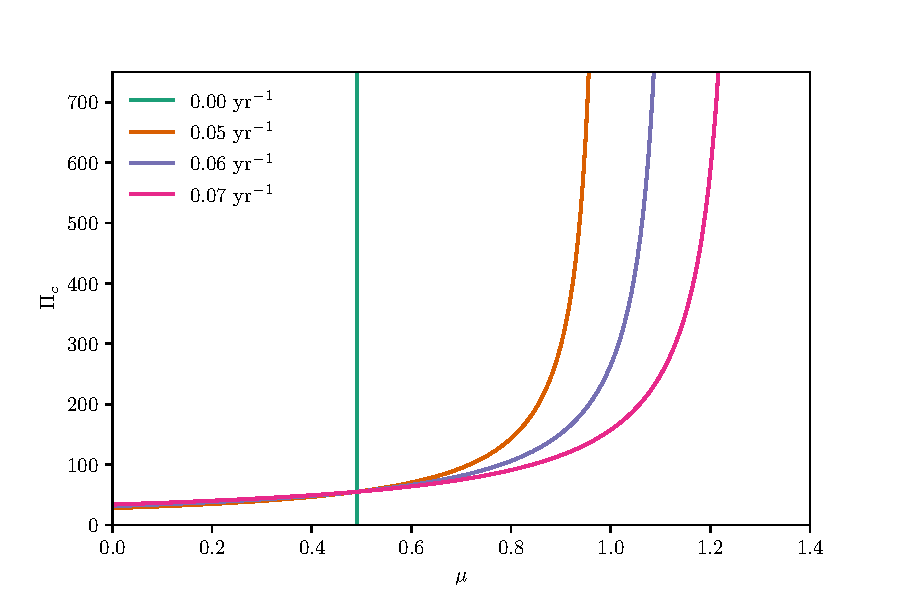
\includegraphics[width=\textwidth,keepaspectratio]{bifurcation_parameter_plane}
  \caption[The ($\mu$,$\Pi_c)$ parameter plane]{A plot of the $(\mu,\Pi_c)$ parameter plane, where the lines are drawn according to \cref{eq:critical_mu_simple_ocean_in_terms_of_npp}
    for a range of different $\dv*{\Pi}{C_a}$ values. The lines separate the stable and unstable regions such that stable regions are to the left of the lines.
    The other parameters are $\chi_0 = 0.25$,$\Pi_0 =\SI{55}{\peta\gram\carbon\per\year}$,
    $C_{a0} = \SI{589}{\peta\gram\carbon}$ and $C_{s}^{\mathrm{eq}} = \SI{1500}{\peta\gram\carbon}$.}
  \label{fig:critical_mu_vs_pic}
\end{figure}


\subsection{Numerical Determination of Bifurcation Diagram}

To numerically compute the equilibria of \cref{eq:global_soil_carbon}, the dependence of $\Pi$ on
$C_a$  must be set. It is chosen to be
\begin{equation}
  \label{eq:npp_fertilization}
  \Pi(C_a) = \frac{\Pi_{\infty} C_a}{C_a + C_{1/2}},
\end{equation}
which is the same choice as~\cite{Cox2006}. The parameter $C_{1/2}$ determines the strength of the \ce{CO2} fertilisation effect. The value of $\Pi_{\infty}$
represents the saturation value of NPP at high \ce{CO2} levels. As the pre-indsutrial NPP, $\Pi_0$, is more accurately known than the saturation value,
$\Pi_{\infty}$  can be determined from $\Pi_0$ using
the formula
\begin{equation}
  \label{eq:npp_saturation_from_pi}
  \Pi_{\infty} = \Pi_0 \frac{C_{a0} + C_{1/2}}{C_{a0}}.
\end{equation}


It is now straightforward to compute the bifurcation diagram, which is plotted in \cref{fig:compost_bomb_bif}. The figure shows the equilibrium soil carbon as a function
of $\mu$ for different values of $\Pi_c$. It can be seen that there is a transcritical bifurcation at a certain value of $\mu$. This value of $\mu$ decreases with decreasing $\Pi_c$.
The numerical calculations also reveal a stable state with large amounts of soil carbon in addition to the pre-industrial state for large enough values of $\mu$. The calculations in
\cref{sec:computation_of_bifurcation_point} are performed by linearising about the pre-industrial state and as such apply only to that state, which is most scientificially relevent.


\begin{figure}
  \centering
  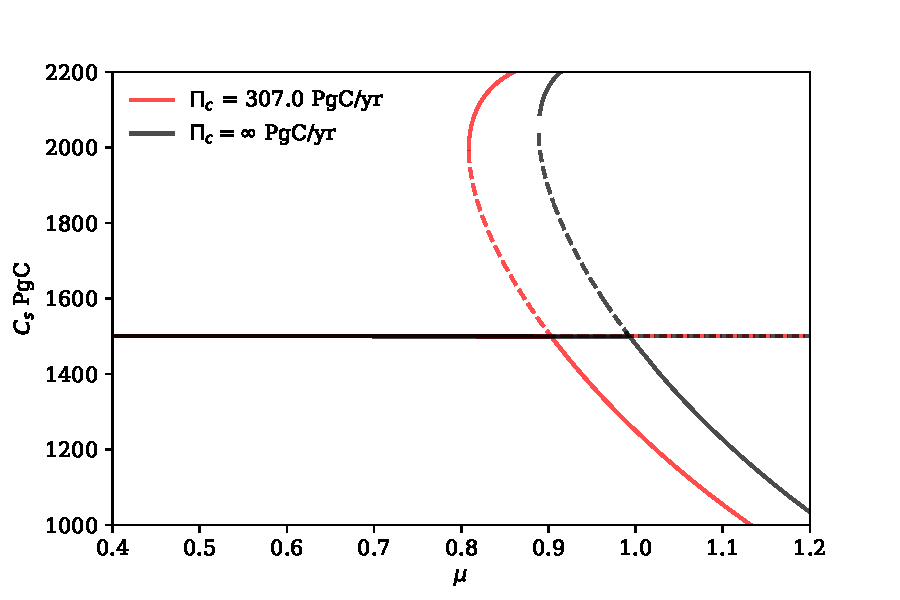
\includegraphics[width=\textwidth,keepaspectratio]{compost_bomb_global_bifurcation}
  \caption[Global Compost Bomb Bifurcation Diagram]{The equilibrium state of \cref{eq:global_soil_carbon} for two values of $\Pi_c$ as a function of $\mu$.
    The two values of $\Pi_c$ represent a no biogeochemical heating case ($\Pi_c = \infty$) and a biogeochemical heating case ($\Pi_c = \SI{308}{\peta\gram\carbon\per\year}$).
    The other parameters were set to $\chi_0 = 0.25$, $\Pi_0 =\SI{55}{\peta\gram\carbon\per\year}$, $C_{1/2} = \SI{593.6}{\peta\gram\carbon}$, $C_{a0} = \SI{589}{\peta\gram\carbon}$,
    $C_{s}^{\mathrm{eq}} = \SI{1500}{\peta\gram\carbon}$.}
  \label{fig:compost_bomb_bif}
\end{figure}

\section{Determining the Parameters}
\subsection{The Effective Climate Sensitivity, $S$}
A first guess to the value of $S$ may be the Equilibrium Climate Sensitivity, ECS, namely the increase in global mean surface temperatures when atmospheric \ce{CO2} concentrations
are doubled \parencite{Sherwood2020}. However, the pattern of warming is spatially heterogeneous, with more warming happening over
land than over oceans \parencite{Morice2021}. As soil carbon is found on land not
in the oceans, it may be better to view $S$ as the climate sensitivity over land.

In order to determine what $S$ should be, the soil carbon balance will be considered at every point on the Earth's surface. There will be a spatially varying amount of warming which will
lead to a change in global soil carbon. This will then be compared to what level of spatially uniform warming would be required to give the same change in soil carbon. By setting the spatially varying
pattern of warming to the pattern of warming caused by doubling \ce{CO2}, the resulting effective warming will be $S$.

Ignoring the effects of biogeochemical heating, the spatially resolved soil carbon balance can be written as:
\begin{equation}
  \label{eq:spatially_resolved_soil_carbon}
  \pdv{C_s(\bm{r},t)}{t} = \Pi(\bm{r},t) - r_0(\bm{r},t)C_s(\bm{r},t)e^{\alpha T_a(\bm{r},t)},
\end{equation}
where $\bm{r}$ is the position on the Earth's surface and $\Pi$, $r_0$ and $C_s$ are allowed to vary spatially. It is assumed that $\alpha$ is constant and that there is no
horizontal transport of soil carbon.

\Cref{eq:spatially_resolved_soil_carbon} can be averaged over space. Denoting spatial averages with $\langle \bullet \rangle$, this gives
\begin{equation}
  \label{eq:spatially_averaged_soil_carbon}
  \dv{\left\langle C_s\right\rangle}{t} = \left\langle \Pi \right \rangle - \left\langle r_0 C_s e^{\alpha T_a} \right \rangle.
\end{equation}
Assuming the warming is small, the exponential can be expanded to first order using $e^x \approx 1 + x$. This will not affect the behaviour of the model
as long as $\alpha T_a \ll 1$. Assuming $Q_{10} = 2$, this requires that $T_a \ll \SI{33}{\kelvin}$, which is the case for realistic amounts of climate change.
This approximation leads to
\begin{align*}
  \dv{\left\langle C_s\right\rangle}{t} &\approx \left\langle \Pi \right \rangle  + \left\langle r_0 C_s + r_0 C_s \alpha T_a \right \rangle \\
                                        &\approx \left\langle \Pi \right \rangle - \left\langle r_0 C_s\right \rangle - \alpha \left \langle r_0C_s T_a\right\rangle.
\end{align*}
Globally averaged respiration must balance globally averaged NPP in equilibrium, so $\langle \Pi \rangle = \langle r_0 C_s \rangle$. Assuming that
temperature change happens faster than changes in NPP and soil carbon, those terms can be approximated with their $T_a = 0$ equilibrium values, giving
\begin{equation}
  \label{eq:soil_carbon_linearised}
  \dv{\langle C_s\rangle}{t} \approx -\alpha \langle \Pi T_a \rangle.
\end{equation}
Introducing an effective temperature $T_{\mathrm{eff}}$, defined so that
\begin{equation}
  \label{eq:motivation_of_effective_temperature}
  - \alpha \left \langle \Pi T_a \right\rangle = - \alpha \left \langle \Pi \right\rangle T_{\mathrm{eff}}
\end{equation}
which implies
\begin{equation}
  \label{eq:definition_of_effective_temperature}
  T_{\mathrm{eff}} = \frac{\left \langle \Pi T_s \right\rangle}{\left \langle \Pi \right\rangle}.
\end{equation}
After a doubling of \ce{CO2}, $T_{\mathrm{eff}} = S$ and $\langle T_a \rangle = \mathrm{ECS}$ which means that
\begin{equation}
  \label{eq:S_vs_ECS}
  \frac{S}{\mathrm{ECS}} = \frac{\left \langle \Pi T_a \right\rangle}{\left \langle \Pi \right\rangle \left \langle T_a \right \rangle}.
\end{equation}
In words, this means $S$ is given by an NPP weighted average of global temperatures. A simple estimate of this ratio can be made by noting that $\Pi$ is zero over ocean.
Assuming that over land the correlation between NPP and $T_a$ is weak then
\begin{equation}
  \label{eq:S_vs_ECS_land_ocean}
  \frac{S}{\mathrm{ECS}}
  = \frac{\left\langle \Pi\right\rangle_{\mathrm{land}} \left\langle T_a \right\rangle_{\mathrm{land}}}{\left \langle \Pi \right\rangle_{\mathrm{land}} \left \langle T_a \right \rangle_{\mathrm{global}}}
  = \frac{\left\langle T\right\rangle_{\mathrm{land}}}{\left\langle T \right\rangle_{\mathrm{global}}}
\end{equation}
which means that $S$ is the climate sensitivity over land, as predicted by the rough guess. The IPCC find that there has been about $1.5$ times more warming over land than over the globe
as a whole \parencite{AR6}.

\Cref{eq:S_vs_ECS} can be used with abrupt-4xCO2 CMIP runs \parencite{Eyring2016} to estimate $S$. Taking $\Pi$ to be the initial NPP in these simulations gives an estimate of $S$ of around $1.5$,
as will be shown in \cref{tab:S_vs_ECS}.

\subsection{The influence of biogeochemical heating, $\Pi_c$}
The quantity $\Pi_c$, which measures the role of biogeochemical heating on the global carbon cycle depends on the sensitivity of heterotrophic respiration to
temperature, the heat released by respiration and the heat transfer coefficient between the land and the atmosphere.

The first of these, $\alpha$, is reasonably well known. In terms of $Q_{10}$ it is $\alpha = 0.1 \log Q_{10}$. $Q_{10}$ is usually taken to be about $2$
\parencite{Jones2001,Clark2011}. This means that $\alpha \approx 0.07$.

The second quantity, $A$, can be estimated biochemically. Its value is taken to be $A = \SI{3.9E7}{\joule\per\kilo\gram\carbon}$ \parencite{Luke2011}.

The final quantity to estimate is the heat transfer coefficient between the land and the atmosphere. This varies from region to region, depending on the land surface cover
\parencite{Beringer2001}, the soil hydrology \parencite{Dharssi2009} and the soil type \parencite{Best2011}. As such an effective heat transfer coefficient will be required.

The heat transfer coefficient can be estimated from the conductivity via
\begin{equation}
  \label{eq:conductivity_via_heat_transfer}
  \kappa = \frac{2\lambda}{\Delta z}
\end{equation}
where $\Delta z$ is a soil thickness and $\lambda$ is the conductivity. Taking $\Delta z = \SI{0.1}{\meter}$ and $\lambda = \SI{0.227}{\watt\per\meter\per\kelvin}$
\parencite{Cox1999} gives a value of $\kappa = \SI{4.5}{\watt\per\meter\squared\per\kelvin}$ and a value of $\Pi_c = \SI{8000}{\peta\gram\carbon\per\year}$. This value is much larger than typical
values of NPP and so this biogeochemical heating effect must be small at the global scale. However, it should be noted that $\kappa$ can be smaller in, for example, well insulated mossy soils
and as such the biogeochemical heating may still be significant regionally.

\section{Conclusions}
In this chapter, I have investigated the role of biogeochemical heating at the global scale. I have shown how the terrestrial carbon cycle is only stable
for a certain parameter range, and that biochemical heating reduces the maximum carbon-climate system sensitivity compatible with a stable carbon cycle.

There are a number of deficiencies with this modelling approach. Firstly, the representation of the ocean is very simple and does not capture any dynamic features of the ocean carbon
cycle. This is an issue taken up in \cref{chapter:conceptual_carbon_cycle}. Furthermore, this chapter only looks at the compost bomb at the global scale, whereas it is
more likely to be important regionally where $\kappa$ and thus $\Pi_c$ values may be substantially smaller. However there is no reason to believe the dependencies
on climate-carbon system sensitivity and the \ce{CO2} fertilisation effect would not hold at the regional as well as the global scale.  
